% Part 2 chapter carrying "On the Dual-Sector Structure of IAM" (Mahaffey, March 2026, informal note), read in full 2026-10-02 (all 573 lines), in its order.
% Checks: docs/verification/chains/DUAL_SECTOR_NOTE_CHECK.md. Figures 1-2 of the note are pre-chain and not carried; chain values are used.
\chapter{Why matter and light are in different sectors}\label{ch:dsnote}

\section{Two kinds of worldline}
General relativity treats massive particles and photons differently at the level of the metric. A massive particle moves on a timelike worldline and accumulates
proper time,
\begin{equation}
g_{\mu\nu}\frac{dx^\mu}{d\tau}\frac{dx^\nu}{d\tau}=-1,\qquad d\tau>0,
\end{equation}
while a photon moves on a null worldline and accumulates none,
\begin{equation}
g_{\mu\nu}\frac{dx^\mu}{d\lambda}\frac{dx^\nu}{d\lambda}=0,\qquad d\tau=0 .
\end{equation}
This is the causal structure of spacetime, not an approximation. Rest mass, $E=mc^2$, is energy bound into a configuration that moves on timelike worldlines; a photon carries energy on a null one.

The sector split follows from one statement: a process that needs a finite proper-time interval $\Delta\tau>0$ to complete cannot run on a worldline with
$\Delta\tau=0$. Gravitational decoherence --- the irreversible production of classical records during structure formation --- is such a process. Photons
therefore cannot take part in it, and the record entropy $S_{\rm info}$ that drives the IAM modification is produced by the matter sector alone.

\section{What a constant term cannot describe}
$\Lambda$ is a property of the geometry: uniform, isotropic, time-independent, and the same for null and timelike geodesics. It is the correct description of the
vacuum baseline. What it cannot describe is a contribution that depends on what matter does --- irreversible decoherence events, the records they leave,
their encoding on the horizon, the resulting change in expansion, and the dilution that slows further collapse. $\Lambda$CDM works well because the record term
$\beta_mE(a)$ is smooth and, over the redshifts where data are most precise, its integrated effect resembles a slowly varying constant. A constant, however, has
no link to when structure forms; in IAM the record term grows with structure formation, so it becomes important when matter is most active. The ingredients ---
Landauer (1961)~\cite{Landauer1961}, Bekenstein--Hawking (1973)~\cite{Bekenstein1973,Hawking1975}, Jacobson (1995)~\cite{Jacobson1995} and decoherence theory (Zurek, 1980s)~\cite{Zurek1981,Zurek1982} --- were developed separately; IAM combines them.

\section{The sector split in the first law}
IAM modifies the Jacobson--Cai--Kim first law~\cite{Jacobson1995,CaiKim2005} of the apparent horizon to
\begin{equation}
-dE=T_H\,d\!\left(S_{\rm geo}+S_{\rm info}\right),
\end{equation}
with $S_{\rm geo}=A_H/4G$ and $S_{\rm info}$ the classical information produced by gravitational decoherence, encoded at Landauer cost $k_BT_H\ln2$ per bit. The
sector split enters through one condition,
\begin{equation}
S_{\rm info}>0\iff d\tau>0 .
\end{equation}
For photons $S_{\rm info}=0$, the first law takes its standard form and general relativity is recovered. In the $\mu$--$\Sigma$ language,
\begin{equation}
\mu(a)=\frac{H^2_{\Lambda{\rm CDM}}(a)}{H^2_{\Lambda{\rm CDM}}(a)+\beta_mE(a)H_0^2}<1,\qquad\Sigma(a)=1,
\end{equation}
with $E(a)=\exp(1-1/a)$ and $\beta_m=\Omega_m/2=0.15765$ from the virial partition --- no parameter beyond $\Lambda$CDM.

$\Sigma=1$ with $\mu\neq1$ also occurs elsewhere: in $f(R)$ gravity, in the quasi-static regime, lensing is unmodified and $\mu$ lies between $1$ and $4/3$~\cite{PogosianSilvestri2008}.
What is specific to IAM is the sign and form of $\mu(a)$ with its amplitude fixed in advance by $\Omega_m/2$, so that $\mu(0)=0.864$ is a prediction, not a fit.

\section{The record so far}
\begin{itemize}
\item Seventeen converged chains on the dual-sector term (12 MGCAMB, 3 modified CAMB, 2 background diagnostics; Chapters~\ref{ch:latetime}, \ref{ch:level2}); with the baryon chain (Chapter~\ref{ch:baryon}), eighteen in all (Chapter~\ref{ch:dual}).
\item Planck: $\Delta\chi^2=+0.54$ at the best points against $\Lambda$CDM with the same parameter count (likelihood ratio $0.76$).
\item $\sigma_8$ from $0.809$ to $0.800$, toward the KiDS-1000, DES~Y3 and HSC~Y3 values~\cite{Asgari2021,DESY3,HSCY3}.
\item $H_0^{(\gamma)}=67.16\pm0.47$ ($-0.37\sigma$ from Planck~\cite{Planck2018VI}); $H_0^{(m)}=72.26$ ($-0.75\sigma$ from SH0ES~\cite{Riess2022}).
\item The same term in the background Friedmann equation gives $H_0\approx61.5$, $10.9\sigma$ from Planck: the modification acts on the perturbations.
\item Photon coupling: fitted to the acoustic scale, $\beta_\gamma<0.0039$ (95\,\%), so $\beta_\gamma/\beta_m<0.025$ \measured\ (Chapter~\ref{ch:dsvalidation}).
\item Supernovae: their distances follow $\Lambda$CDM geometry; the $\beta$ term applied to them is excluded ($\Delta\chi^2=+23.6$; Chapter~\ref{ch:dsvalidation}) \measured.
\item In the Planck chain, $\Omega_m/2=0.1583\pm0.0033$, $0.2\sigma$ from the fixed $\beta_m$.
\end{itemize}
Whether the DESI preference for evolving dark energy~\cite{DESI2025} arises from fitting one fluid to $\Lambda$CDM distances together with slower growth is a test still to be done
on real data with two rulers (Chapter~\ref{ch:sectortension}).

\section{What would count against the dual-sector structure}

\begin{figure}[htbp]\centering
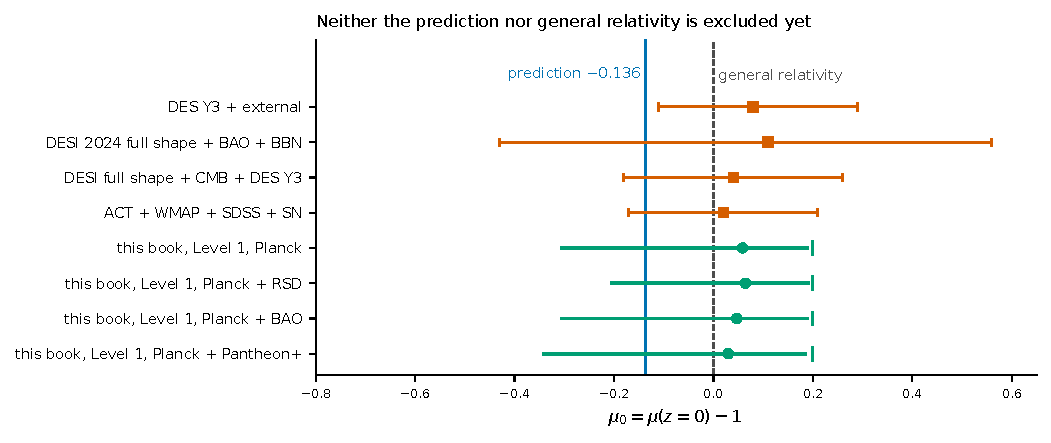
\includegraphics[width=\textwidth]{figures/part2/fig_mu0_constraints.pdf}
\caption{Constraints on $\mu_0=\mu(z{=}0)-1$. Squares: published values as quoted in Chapter~\ref{ch:latetime} (68\,\% intervals): DES Y3 with external data $0.08^{+0.21}_{-0.19}$; DESI 2024 full shape with BAO and BBN $0.11^{+0.45}_{-0.54}$; DESI full shape with CMB and DES Y3 $0.04\pm0.22$; ACT + WMAP + SDSS + SN $0.02\pm0.19$ \observed. The prediction lies 1.14, 0.46, 0.80 and $0.82\sigma$ from them, general relativity within $0.42\sigma$. Circles: this book's Level~1 chains with $\mu_0$ free (flat prior $[-0.5,+0.2]$, the tick marks its upper edge), median and central 90\,\% interval, from the chain files \measured. Vertical line: the prediction $\mu_0=-0.136$ \prediction. The published values are for the template $\mu(z)=1+\mu_0\,\Omega_{\rm DE}(z)/\Omega_{\rm DE}(0)$, whose deviation lasts to higher redshift than IAM's; matched in growth, the IAM $\mu(z)$ corresponds to $\mu_0\approx-0.07$ in that template (Section~\ref{sec:lt_euclid}) \calc, so the distances quoted for $-0.136$ overstate the separation.}\label{fig:mu0_constraints}
\end{figure}
\begin{itemize}
\item $\Sigma\neq1$ detected by Euclid tomography~\cite{Euclid2025}: the photon exemption would fail.
\item $\beta_\gamma>0$ detected by CMB-S4~\cite{Abazajian2016}: photons would be coupled.
\item $\Omega_m$ revised while the growth data still require the old $\beta_m$: the virial ratio $\beta_m/\Omega_m=1/2$ would fail.
\item Scale-dependent $\mu$ or $\Sigma$: in IAM both depend on redshift only.
\end{itemize}
Euclid, DESI Year~5 and CMB-S4 test each of these.
